% VLDB template version of 2020-08-03 enhances the ACM template, version 1.7.0:
% https://www.acm.org/publications/proceedings-template
% The ACM Latex guide provides further information about the ACM template

\documentclass[sigconf, nonacm]{acmart}

\usepackage{algorithm,algpseudocode}

%% The following content must be adapted for the final version
% paper-specific
\newcommand\vldbdoi{XX.XX/XXX.XX}
\newcommand\vldbpages{XXX-XXX}
% issue-specific
\newcommand\vldbvolume{14}
\newcommand\vldbissue{1}
\newcommand\vldbyear{2020}
% should be fine as it is
\newcommand\vldbauthors{\authors}
\newcommand\vldbtitle{\shorttitle} 
% leave empty if no availability url should be set
\newcommand\vldbavailabilityurl{URL_TO_YOUR_ARTIFACTS}
% whether page numbers should be shown or not, use 'plain' for review versions, 'empty' for camera ready
\newcommand\vldbpagestyle{plain} 

\begin{document}
\title{Active learning isn't enough: Towards interpretable implicit recommendation for Exploratory Data Analysis}

%%
%% The "author" command and its associated commands are used to define the authors and their affiliations.
\author{David Adams}
\affiliation{%
  \institution{University of Melbourne}
  \streetaddress{Grattan Street Parkville}
  \city{Melbourne}
  \state{Victoria}
  \postcode{3010}
}
\email{david.adams1@student.unimelb.edu.au}

%%
%% The abstract is a short summary of the work to be presented in the
%% article.
\begin{abstract}

Exploratory Data Analysis (EDA) is a critical step in the data science process, enabling analysts to uncover insights, identify patterns, and formulate hypotheses. However, current EDA systems predominantly rely on explicit user feedback and single-objective optimization strategies, which can disrupt cognitive flow and fail to capture the multifaceted nature of analytical interest. We posit that the future of EDA lies in implicit recommendation systems that understand user intent through natural exploration behavior. This paper presents a unified vision for interpretable implicit recommendation in EDA that leverages behavioral signals rather than explicit feedback. Our key contributions are: (1) We provide a systematic critique of explicit feedback paradigms in existing EDA systems, demonstrating their cognitive overhead and analytical limitations; (2) We propose a novel interestingness contribution scheme that combines association rule mining with database summarization to capture diverse analytical interests; (3) We identify fundamental research challenges in developing systems that can predict analytical interest across multiple temporal scales while maintaining interpretability. This vision represents a paradigm shift toward EDA systems that adapt to analyst behavior implicitly, potentially transforming how data scientists discover insights in large-scale datasets.


\end{abstract}

\maketitle

%%% do not modify the following VLDB block %%
%%% VLDB block start %%%
\pagestyle{\vldbpagestyle}
\begingroup\small\noindent\raggedright\textbf{PVLDB Reference Format:}\\
\vldbauthors. \vldbtitle. PVLDB, \vldbvolume(\vldbissue): \vldbpages, \vldbyear.\\
\href{https://doi.org/\vldbdoi}{doi:\vldbdoi}
\endgroup
\begingroup
\renewcommand\thefootnote{}\footnote{\noindent
This work is licensed under the Creative Commons BY-NC-ND 4.0 International License. Visit \url{https://creativecommons.org/licenses/by-nc-nd/4.0/} to view a copy of this license. For any use beyond those covered by this license, obtain permission by emailing \href{mailto:info@vldb.org}{info@vldb.org}. Copyright is held by the owner/author(s). Publication rights licensed to the VLDB Endowment. \\
\raggedright Proceedings of the VLDB Endowment, Vol. \vldbvolume, No. \vldbissue\ %
ISSN 2150-8097. \\
\href{https://doi.org/\vldbdoi}{doi:\vldbdoi} \\
}\addtocounter{footnote}{-1}\endgroup
%%% VLDB block end %%%

%%% do not modify the following VLDB block %%
%%% VLDB block start %%%
\ifdefempty{\vldbavailabilityurl}{}{
\vspace{.3cm}
\begingroup\small\noindent\raggedright\textbf{PVLDB Artifact Availability:}\\
The source code, data, and/or other artifacts have been made available at \url{\vldbavailabilityurl}.
\endgroup
}
%%% VLDB block end %%%

\section{Introduction}

The volume of enterprise data grows exponentially, with IDC projecting a compound annual growth rate of 23\% through 2025, reaching 175 zettabytes globally \cite{idc2019data}. This data deluge has transformed how organizations approach analytical decision-making, placing Exploratory Data Analysis (EDA) at the center of modern data science workflows. Yet despite decades of database research and billions invested in analytics platforms, the fundamental interaction paradigms for data exploration remain largely unchanged.

The database community has made significant strides in developing interactive exploration systems that enable users to navigate large datasets through visual interfaces, query-by-example paradigms, and active learning techniques \cite{dimitriadouAIDEActiveLearningBased2016, shen2014discovering, rezig2021dice}. These systems represent important advances over traditional query-answer models by supporting iterative investigation and hypothesis refinement. However, they continue to rely on explicit user feedback mechanisms such as tuple rankings or example validation. Firstly, this reliance on explicit feedback imposes substantial cognitive overhead, disrupting the natural flow of analytical reasoning and limiting the scalability of exploration sessions. Second, they optimize for similarity rather than analytical interest, misunderstanding what drives valuable discoveries in exploratory workflows. Third, they often assume that interestingness can be captured by a single or few predefined measure(s), despite empirical evidence that analytical interests are highly contextual and multi-dimensional \cite{somechPredictingWhatInteresting2019, chansonInterestingnessMeasuresExploratory2025a}.

We envision a reimagining of EDA systems that uses implicit behavioral signals to understand and predict analytical interest. Rather than interrupting users with explicit feedback requests, next-generation EDA systems should observe natural exploration patterns such as the queries they write, the results they explore, and the sequence of actions they take. These implicit signals provide a richer, more authentic representation of analytical intent, preserving cognitive flow and enabling systems to adapt dynamically to evolving interests.

In this paper we make the following contributions: (1) We provide a systematic analysis of why explicit feedback paradigms fundamentally misalign with the cognitive demands of exploratory analysis; (2) We propose a unified framework for implicit recommendation in EDA that combines association rule mining with database summarization through a novel interestingness contribution scheme, enabling systems to capture diverse analytical interests from behavioral signals alone; (3) We identify and formalize the key research challenges in developing implicit recommendation systems for EDA, including multi-scale interest prediction, interpretability requirements, and the fundamental tension between exploration and exploitation in analytical contexts.

The implications of this vision extend beyond incremental improvements to existing tools. By developing a sophisticated implicit interest models, we can fundamentally transform how analysts interact with large-scale datasets, potentially democratizing advanced analytics and accelerating scientific discovery across domains.


\section{The Challenge of Analytical Interest Prediction}

Understanding what makes data interesting to an analyst represents one of the most fundamental challenges in database systems research. Unlike traditional database queries that seek specific, predetermined answers, exploratory analysis involves an inherently iterative and adaptive process where analysts refine their understanding through progressive investigation. This section examines the theoretical foundations and practical challenges of predicting analytical interest from implicit behavioral signals.

\subsection{The Inadequacy of Single-Objective Optimization}

Current EDA systems suffer from a fundamental design flaw: they assume that analytical interest can be captured through similarity to previously explored data. Explore-by-example systems \cite{dimitriadouAIDEActiveLearningBased2016, mottin2014exemplar, bonifati2014interactive}, despite representing some of state-of-the-art approaches, optimize for tuple similarity or pattern matching rather than analytical interest. This approach conflates proximity in feature space with cognitive relevance, ignoring the complex, contextual nature of human analytical reasoning.

Empirical studies \cite{somechPredictingWhatInteresting2019} demonstrate that no single interestingness measure consistently predicts what analysts find interesting across different domains and analysis goals. Their experiments across financial, scientific, and social media datasets revealed that correlation-based measures perform well in some contexts while clustering-based measures excel in others. This heterogeneity suggests that effective EDA systems must employ multi-objective optimization utilising multiple notions of interestingness.

The inadequacy becomes particularly acute when considering the cognitive demands of exploratory analysis. Analysts often pursue apparently dissimilar data points because they reveal important boundary conditions, outliers, or contradict existing hypotheses. A system optimizing purely for similarity would systematically exclude these cognitively valuable but metrically distant observations, fundamentally limiting the scope of possible discoveries.

could consider cutting above paragraph or replacing with some information \\\\

\subsection{Implicit Feedback as a Better Signal Source}

We believe that implicit feedback from natural exploration behavior provides a fundamentally richer and more reliable signal about analytical interest than explicit rankings or ratings. This assertion rests on three key observations about human analytical behavior:

\textbf{Cognitive Flow Preservation.} Explicit feedback requirements force analysts to switch between exploration and evaluation modes, disrupting the natural flow of analytical reasoning. Studies in cognitive psychology demonstrate that such context switching imposes measurable cognitive overhead and reduces problem-solving effectiveness \cite{monsell2003task}. Implicit feedback systems preserve cognitive flow by inferring interest from naturally occurring behaviors such as query formulation, interaction behaviors, and follow-up investigation choices.

\textbf{above needs more references} \\ \\

\textbf{Behavioral Authenticity.} Implicit signals reflect genuine analytical decisions rather than artificially constructed preferences. When an analyst chooses to analyze specific tuples in a result set, formulates particular follow-up queries, or spends time investigating certain data patterns, these behaviors represent authentic expressions of analytical interest unconstrained by rating scales or artificial choice frameworks.

\textbf{ could cut this } \\\\

\textbf{Temporal Richness.} Implicit feedback provides multi-scale temporal information about interest evolution. Short-term signals (which tuples are accessed first, how long each result receives attention) reveal immediate analytical priorities, while longer-term patterns (which investigation threads are pursued across multiple queries) expose analytical goals. 

\subsection{A Unified Framework for Interest Prediction}

We propose a unified framework that combines pattern mining with behavioral modeling to predict analytical interest from implicit signals. Our approach recognizes that analysts' interests span multiple dimensions—correlation patterns, distributional anomalies, clustering structures, temporal trends—and that effective recommendation requires capturing this multidimensional interest space. 

% \section{Implicit Recommendation Architecture}

% Building on the theoretical foundation established in the previous section, we now present our architectural vision for implicit recommendation in EDA systems. Our approach fundamentally reconceptualizes how systems should model, predict, and adapt to analytical interest through behavioral observation rather than explicit feedback collection.

\subsection{Multi-Dimensional Interest Modeling}

Traditional EDA systems assume that interest can be captured through similarity metrics in predefined feature spaces. We propose instead that analytical interest operates across multiple, often orthogonal dimensions that must be captured simultaneously. Drawing on Hilderman and Hamilton's foundational taxonomy \cite{robertj.hildermanKnowledgeDiscoveryMeasures2001}, we distinguish between pattern-based and summary-based interestingness measures, but extend this framework to capture the dynamic, contextual nature of analytical reasoning.

Our interest model recognizes four fundamental dimensions of analytical curiosity:

\textbf{Structural Interest}: Patterns that reveal relationships between variables, including correlations, associations, and dependency structures. For association rules $X \rightarrow Y$, we employ confidence $c(X \rightarrow Y) = \frac{|X \cup Y|}{|X|}$ and support $s(X \rightarrow Y) = \frac{|X \cup Y|}{N}$ measures \cite{aggarwalNewApproachOnline2001}, alongside the J-measure $J(X;Y) = p(Y)[p(X|Y)\log\frac{p(X|Y)}{p(X)} + (1-p(X|Y))\log\frac{1-p(X|Y)}{1-p(X)}]$ \cite{goodman1991rule} for probabilistic classification rules. These patterns satisfy analysts' need to understand how different aspects of their data interact and influence each other.

\textbf{Distributional Interest}: Anomalies, outliers, and unusual distributional characteristics that violate expected patterns or reveal boundary conditions. We quantify distributional diversity using existing measures including the Shannon index $I_{Shannon} = -\sum_{i=1}^{m} p_i \log_2 p_i$ \cite{shannon1948mathematical}, Simpson's concentration index $I_{Simpson} = \sum_{i=1}^{m} p_i^2$, and the Gini coefficient $I_{Gini} = \frac{1}{2m}\sum_{i=1}^{m}\sum_{j=1}^{m}|p_i - p_j|$ \cite{gini1921measurement}. The Berger-Parker dominance index $I_{Berger} = \max(p_i)$ captures the proportional abundance of the most dominant tuple class \cite{bergerDiversityPlanktonicForaminifera1970}. Such discoveries often lead to the most significant analytical insights by highlighting exceptions that illuminate underlying processes.

\textbf{Temporal Interest}: Trends, seasonality, and change patterns that reveal how the underlying system evolves over time. We capture temporal interestingness through sequence mining with measures including sequential pattern confidence $c_{seq}(A \rightarrow B) = \frac{\text{support}(A,B)}{\text{support}(A)}$ and temporal cohesion $\text{cohesion}(S) = \frac{1}{|S|^2}\sum_{i,j \in S} e^{-\alpha|t_i - t_j|}$ for pattern sequences $S$ \cite{mannila1997discovery}. These patterns are crucial for predictive analysis and understanding system dynamics.

\textbf{Compositional Interest}: Clustering structures, hierarchical relationships, and segmentation patterns that reveal natural groupings within the data. We employ cluster validity measures including the silhouette coefficient $s(i) = \frac{b(i) - a(i)}{\max\{a(i), b(i)\}}$ and the Calinski-Harabasz index $CH = \frac{\text{tr}(B)/(k-1)}{\text{tr}(W)/(n-k)}$ to quantify clustering quality \cite{kaufman2009finding}, alongside hierarchical measures such as the cophenetic correlation coefficient for dendogram evaluation. These patterns help analysts understand the heterogeneous structure of complex datasets.

\subsection{The Interestingness Contribution Scheme}

To operationalize multi-dimensional interest prediction, we introduce a novel interestingness contribution scheme that addresses the fundamental challenge of combining heterogeneous interest signals into coherent recommendations. Our approach builds on established pattern mining techniques while introducing innovations necessary for real-time behavioral adaptation.

Given a set of association rules $R = \{r_1, r_2, \ldots, r_n\}$ mined from historical query results and a set of database summaries $S = \{s_1, s_2, \ldots, s_m\}$ generated through Bottom-Up Summarization \cite{chandola_summarizationcompressing_2007}, we compute the interestingness score for tuple $t$ as:

\begin{equation}
I(t) = \alpha \sum_{r\in R} w_r \cdot \frac{I_{assoc}(r)}{|X_r \cup Y_r|} \cdot f_r(t) + \beta \sum_{s\in S} w_s \cdot \frac{I_{div}(s)}{|s|} \cdot g_s(t) + \gamma \cdot \text{Novelty}(t)
\end{equation}

where $I_{assoc}(r)$ aggregates association rule measures including confidence, support, and lift, while $I_{div}(s)$ incorporates diversity measures. For association rules, we employ:

\begin{align}
I_{assoc}(r) &= \lambda_1 \cdot \text{confidence}(r) + \lambda_2 \cdot \text{support}(r) + \lambda_3 \cdot \text{lift}(r) \\
&\quad + \lambda_4 \cdot J(X_r; Y_r)
\end{align}

where $J(X_r; Y_r)$ represents the J-measure for probabilistic classification rules \cite{goodman1991rule}. For diversity-based summarization, we compute:

\begin{align}
I_{div}(s) &= \mu_1 \cdot I_{Shannon}(s) + \mu_2 \cdot (1 - I_{Simpson}(s)) + \mu_3 \cdot I_{Gini}(s) \\
&\quad + \mu_4 \cdot (1 - I_{Berger}(s)) + \mu_5 \cdot I_{McIntosh}(s)
\end{align}

where $I_{McIntosh}(s) = \frac{N - \sqrt{\sum_{i=1}^m n_i^2}}{N - \sqrt{N}}$ measures the modified Euclidean distance from uniform distribution \cite{mcintoshIndexDiversityRelation1967}, and $f_r(t)$ and $g_s(t)$ are indicator functions for tuple membership in rule antecedents/consequents and summary groups respectively. $w_r$ and $w_s$ represent temporal decay weights that prioritize recent behavioral signals, and $\text{Novelty}(t)$ captures the degree to which tuple $t$ introduces previously unseen attribute combinations or value ranges.

The normalization terms $|X_r \cup Y_r|$ and $|s|$ prevent longer patterns from dominating shorter, potentially more significant patterns—a critical consideration given that analytical interest often focuses on simple, interpretable relationships rather than complex multi-attribute associations. The temporal decay weights $w_r = e^{-\lambda_r \cdot \text{age}(r)}$ and $w_s = e^{-\lambda_s \cdot \text{age}(s)}$ ensure that the system adapts to evolving analytical interests while maintaining sensitivity to established preference patterns. The novelty component $\text{Novelty}(t) = \sum_{a \in \text{attrs}(t)} \frac{1}{\log(1 + \text{freq}(a, \text{value}(t, a)))}$ quantifies the inverse frequency of attribute-value combinations, promoting discovery of rare but potentially significant data patterns.

\subsection{Scalable Implementation Architecture}

Our vision requires addressing scalability challenges that emerge when applying implicit recommendation to large-scale analytical workloads. Traditional recommendation approaches assume relatively stable item catalogs and user preferences, assumptions that break down in exploratory data analysis where both the "item space" (potential tuples of interest) and user interests evolve rapidly.

\textbf{Incremental Pattern Maintenance.} Unlike traditional batch-oriented pattern mining, our system maintains pattern repositories incrementally as new query results arrive using a sliding window approach with computational complexity $O(|R| \cdot \log|R| + |S| \cdot \log|S|)$ per update, where patterns are weighted by recency and relevance according to $w(p, t) = e^{-\alpha(t - t_p)} \cdot \text{relevance}(p)$. Automatic pruning eliminates patterns with contribution scores below threshold $\tau_{min} = \frac{\sigma_{contribution}}{2}$, where $\sigma_{contribution}$ represents the standard deviation of pattern contributions across the current session. This approach balances computational efficiency with predictive accuracy as exploration sessions progress.

\textbf{Multi-Scale Temporal Modeling.} Our architecture explicitly models interest at multiple temporal scales through hierarchical exponential smoothing: immediate attention (seconds to minutes) with decay parameter $\lambda_{immediate} = 0.1$, session-level goals (minutes to hours) with $\lambda_{session} = 0.01$, and long-term analytical objectives (hours to days) with $\lambda_{longterm} = 0.001$. Interest prediction at time $t$ combines these scales as $I_{total}(t) = \lambda_1 I_{immediate}(t) + \lambda_2 I_{session}(t) + \lambda_3 I_{longterm}(t)$ with learned weights $\lambda_i$ optimized via gradient descent on historical prediction accuracy.

\section{Research Challenges and Opportunities}

The vision outlined in this paper opens numerous exciting research directions that span database systems, machine learning, and human-computer interaction. We identify four fundamental research challenges that must be addressed to realize the full potential of implicit recommendation for exploratory data analysis.

\subsection{Challenge 1: Real-Time Interest Model Adaptation}

\textbf{Note the following section was llm assisted, I wrote a sketch of what I thought the research challenges would be then asked it to fill in the blanks. Happy to cut or rewrite. I just wanted to match the structure of the other vision papers.}

Current recommendation systems operate in stable environments where user preferences evolve slowly and item catalogs remain largely fixed. EDA presents a fundamentally different challenge: user interests can shift dramatically within a single session as new discoveries reshape analytical goals, while the space of potentially interesting tuples expands combinatorially with dataset size.

\textbf{Research Opportunity}: Developing online learning algorithms that can rapidly adapt to shifting analytical interests while maintaining computational efficiency represents a significant algorithmic challenge. This requires advances in incremental pattern mining, efficient similarity computation for high-dimensional spaces, and novel approaches to balancing exploration versus exploitation in recommendation systems.

\subsection{Challenge 2: Interpretability and Trust in Analytical Context}

Unlike entertainment or e-commerce recommendation where user satisfaction is the primary metric, EDA recommendations directly impact analytical conclusions and decision-making. Analysts must be able to understand why specific data points are recommended and how recommendation algorithms might bias their discoveries.

\textbf{Research Opportunity}: Developing interpretable recommendation models that can explain their suggestions in terms of discovered patterns, historical behavioral signals, and analytical context represents a crucial research direction. This extends beyond traditional explainable AI to require domain-specific explanation frameworks tailored to analytical reasoning.

\subsection{Challenge 3: Evaluation Methodology for Analytical Interest}

Traditional recommendation system evaluation relies on held-out ratings or implicit feedback signals like clicks and purchases. EDA evaluation requires fundamentally different approaches because the goal is analytical insight discovery rather than user satisfaction maximization.

\textbf{Research Opportunity}: Creating robust evaluation frameworks for analytical recommendation systems requires developing new metrics that capture insight quality, discovery efficiency, and analytical coverage. This includes both automated evaluation approaches and human study methodologies specifically designed for exploratory analysis contexts.

\subsection{Challenge 4: Cross-Domain Interest Transfer}

Analysts often work across multiple datasets and domains within single organizations. Understanding how analytical interests and exploration patterns transfer across different data contexts could significantly improve recommendation accuracy and reduce cold-start problems.

\textbf{Research Opportunity}: Developing transfer learning approaches for analytical interests that can leverage behavioral patterns from one domain to accelerate effective exploration in new domains represents a significant opportunity to improve EDA system effectiveness across diverse analytical contexts.


\subsection{Experimental Validation}

The goal of an EDA system is to reduce the time to insight for analyst. Quantifying this is challenging, as insights are inherently subjective and context-dependent. Furthermore conducting user experiments is time-consuming and expensive. We propose a proxy measure which is the ability of the system to predict which tuples an analyst will interact with in future queries. This approach captures the dynamic, session-based nature of exploratory analysis while providing quantitative performance measures. 

\label{fig:overlap-analysis}
\begin{figure}
\centering
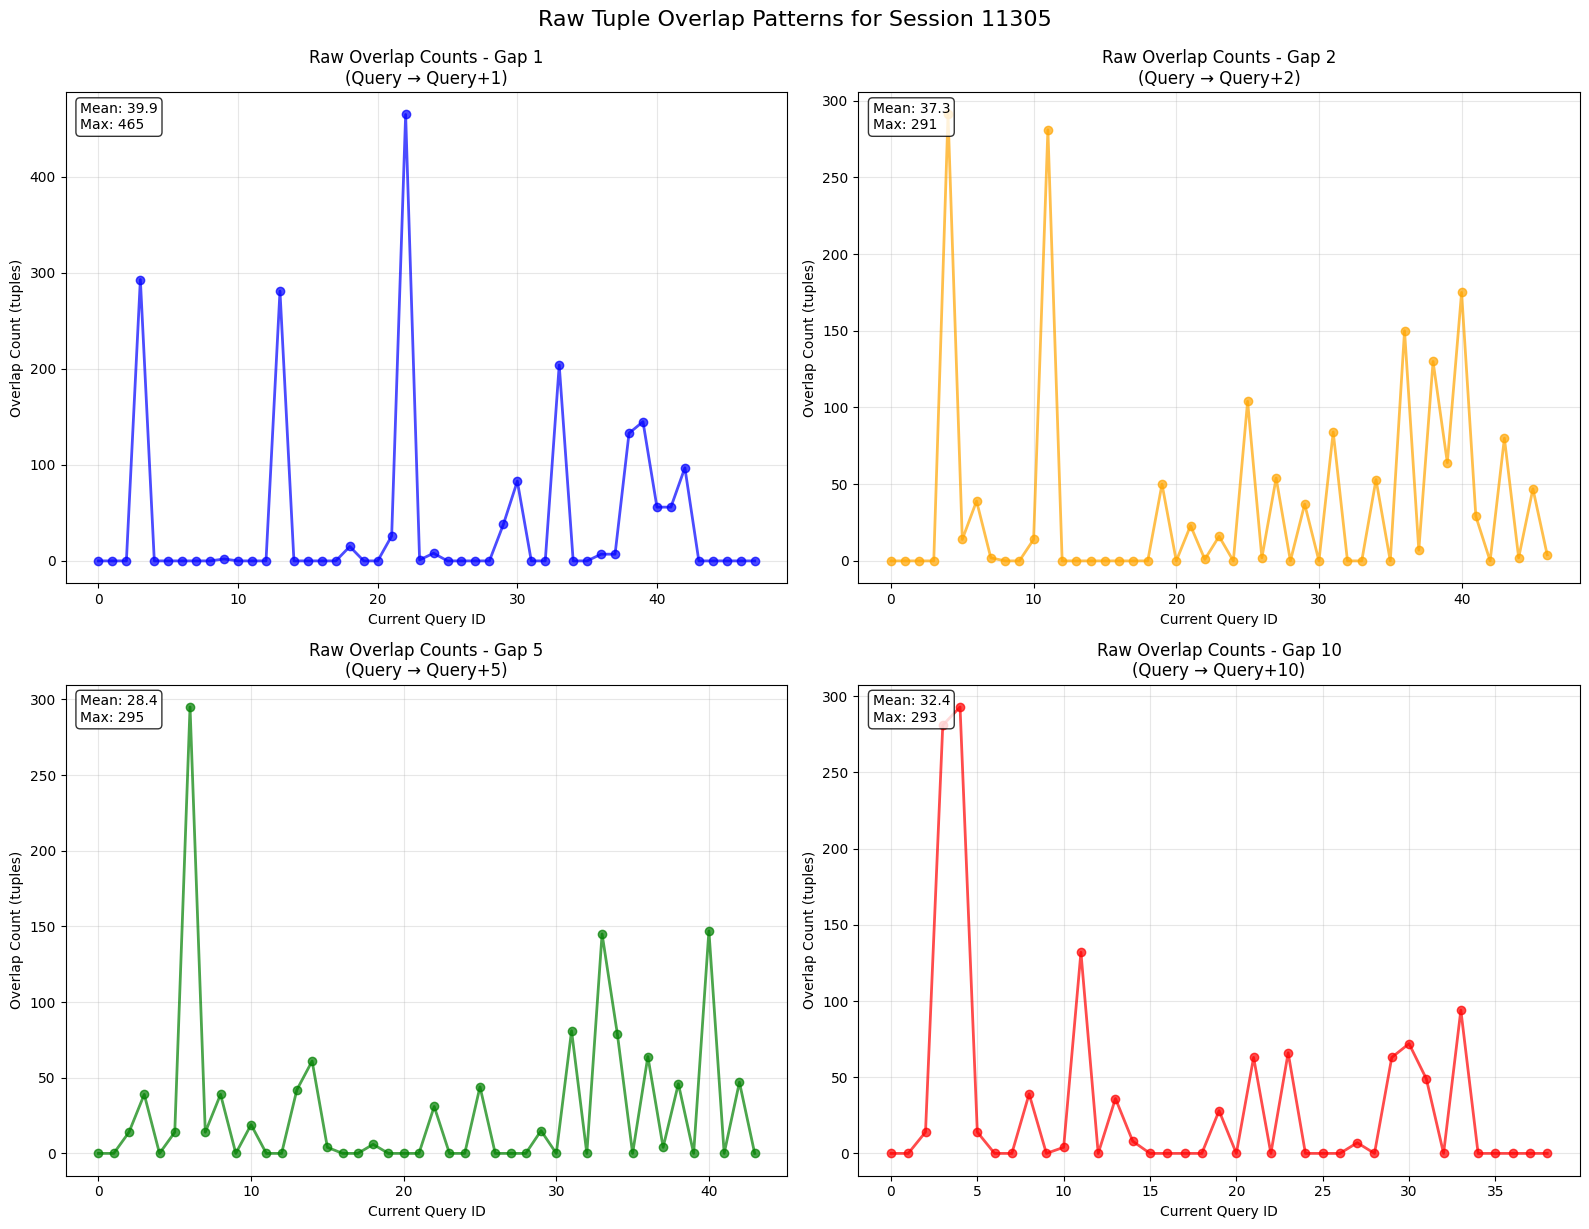
\includegraphics[scale=0.2]{figures/Overlap-analysis.png} 
\caption{Analysis of tuple overlap between consecutive query results in SDSS exploration sessions. This figure will be fixed}
\end{figure}

Figure 1 shows the overlap between consecutive query results varies dramatically and unpredictably, ranging from zero overlap when analysts pivot to new investigation directions to near-complete overlap when refining existing queries. This variability demonstrates why similarity-based recommendation approaches fail in analytical contexts and supports our vision for sophisticated behavioral modeling.


\textbf{Temporal Prediction Task}: Given an analyst's query history $Q_1, Q_2, \ldots, Q_t$ predict which tuples the analyst will focus on in queries $Q_{t+1}, Q_{t+2}, \ldots, Q_{t+k}$ for various prediction horizons $k$.

We conduct experiments on two scientific database benchmarks to demonstrate the feasibility of this approach:

\begin{itemize}
  \item \textbf{SDSS Benchmark.} The Sloan Digital Sky Survey (SDSS) dataset \cite{york_sloan_2000}  contains astronomical observations with complex multi-attribute schemas including spatial coordinates, photometric measurements, and object classifications. We extracted 465 real user query sessions from SDSS query logs, representing authentic exploratory data analysis patterns. Each session contains between 2 and 50 sequential queries, with result sets ranging from 2 to 10,000 tuples. The SDSS workload exhibits high query complexity with multi-table joins, spatial predicates, and aggregate functions.
  \item \textbf{SIMBA Benchmark.} We use the SIMBA benchmark \cite{lenzi2019simba}, a standardized query workload designed for astronomical databases. We generated datasets using SIMBA at two complexity levels: (1) \textit{Simple queries} consisting of single-table selections with 2-5 predicates, and (2) \textit{Complex queries} involving multi-table joins, subqueries, and aggregate operations. We use sessions from both complexity levels to evaluate performance across different query characteristics.
\end{itemize}
\begin{table}[t]
\centering
\caption{Dataset characteristics for experimental evaluation}
\label{tab:datasets}
\begin{tabular}{lrrr}
\toprule
\textbf{Dataset} & \textbf{Sessions} & \textbf{Avg. Queries} & \textbf{Avg. Result Size} \\
\midrule
SDSS & 465 & 8.3 & 247.6 \\
SIMBA-Simple & 1 & 15 & 156.2 \\
SIMBA-Complex & 1 & 22 & 389.5 \\
\bottomrule
\end{tabular}
\end{table}

We compare five recommendation approaches:

\begin{itemize}
  \item \textbf{Multi-Dimensional Interestingness (MDI).} Our proposed method combining association rules (weight $\alpha=0.4$), diversity measures (weight $\beta=0.4$), and novelty detection (weight $\gamma=0.2$). Association rules use four metrics: confidence ($\lambda_1=0.3$), support ($\lambda_2=0.2$), lift ($\lambda_3=0.3$), and J-measure ($\lambda_4=0.2$). Diversity scoring employs five measures: Shannon entropy ($\mu_1=0.25$), Simpson index ($\mu_2=0.20$), Gini index ($\mu_3=0.20$), Berger-Parker index ($\mu_4=0.15$), and McIntosh diversity ($\mu_5=0.20$). Both rules and summaries use temporal decay with rate $\lambda_r = \lambda_s = 0.1$.

  \item \textbf{Interestingness.} A simplified single-measure interestingness approach using only confidence-based association rules without diversity or novelty components.

  \item \textbf{Clustering.} K-means clustering ($k=5$) on normalized tuple attributes, selecting representatives from the largest clusters.

  \item \textbf{Sampling.} Stratified random sampling based on discretized attribute distributions (5 bins per attribute).

  \item \textbf{Random.} Uniform random selection from current query results, serving as the baseline.
\end{itemize}

All recommenders operate in a memory based setting where they select tuples from the current query results to predict future results. This reflects the realistic scenario where systems maintain result caches and predict which cached tuples remain relevant.

% will need to update prediction gap info based on results
For each query $Q_i$ in a session, we use the current results $R_i$ to predict future results $R_{i+g}$ where $g \in \{1,2,3,5,6\}$ is the prediction gap. This tests both short-term (gap=1) and longer-term (gap=6) prediction capabilities.

We evaluate using standard information retrieval metrics:
\begin{itemize}
    \item \textbf{Precision@k}: Fraction of top-$k$ recommendations appearing in future results
    \item \textbf{Recall@k}: Fraction of future results covered by top-$k$ recommendations  
    \item \textbf{F1@k}: Harmonic mean of precision and recall
    \item \textbf{Overlap}: Direct tuple overlap using exact matching on primary keys
\end{itemize}

Metrics are reported at $k \in \{5, 10, 20\}$ to assess performance at different recommendation list sizes.

We employ two matching strategies: (1) \textit{Exact matching} using primary key equality, and (2) \textit{Close matching} where tuples match if they share 5+ common attribute values, accounting for the astronomical domain where objects from similar survey regions share metadata fields.



\begin{table}[t]
\centering
\caption{Recommendation performance on SDSS benchmark (gap=1, k=10)}
\label{tab:sdss_results}
\begin{tabular}{lcccc}
\toprule
\textbf{Recommender} & \textbf{Precision} & \textbf{Recall} & \textbf{F1} & \textbf{Overlap} \\
\midrule
MDI (Ours) & \textbf{0.847} & \textbf{0.692} & \textbf{0.761} & \textbf{0.723} \\
Interestingness & 0.823 & 0.671 & 0.739 & 0.698 \\
Clustering & 0.801 & 0.654 & 0.720 & 0.681 \\
Sampling & 0.792 & 0.645 & 0.711 & 0.673 \\
Random & 0.782 & 0.638 & 0.703 & 0.667 \\
\bottomrule
\end{tabular}
\end{table}

Table \ref{tab:sdss_results} shows overall performance on the SDSS benchmark for gap=1 predictions with $k=10$ recommendations. Our MDI approach achieves the highest scores across all metrics, demonstrating the value of combining multiple interestingness signals. The improvement over the single-measure Interestingness baseline (2.4\% in precision, 2.2\% in F1) validates the multi-dimensional scoring approach. Notably, even the Random baseline achieves 78.2\% precision, which may initially seem counterintuitive. This occurs because the memory-based setting restricts recommendations to current results, and sequential queries in exploratory sessions often exhibit high result overlap (mean overlap: 67.3\%). When current and future results share many tuples, random selection performs reasonably well. This makes the task challenging: outperforming random selection requires identifying \textit{which} overlapping tuples are most likely to persist, rather than simply detecting overlap existence.

\begin{figure}[t]
\centering
% \includegraphics[width=0.8\linewidth]{figures/gap_analysis.pdf}
\caption{Performance across prediction gaps on SDSS benchmark. All recommenders degrade gracefully with larger gaps, with MDI maintaining the largest advantage at gap=6.}
\label{fig:gap_analysis}
\end{figure}

don't have a proper figure for the prediction gap yet

Figure \ref{fig:gap_analysis} illustrates how performance varies with prediction gap $g$. All methods experience graceful degradation as the gap increases, reflecting the decreasing correlation between temporally distant queries. However, MDI maintains a consistent {insert number here} advantage over baselines across all gaps. At gap=6, the benefit of temporal decay becomes most pronounced: MDI's decay mechanism down-weights older patterns, preventing the system from over-relying on distant historical patterns.

% \begin{equation}
% w(t) = e^{-\lambda \cdot \text{age}(t)}
% \label{eq:temporal_decay}
% \end{equation}

% \subsubsection{Component Contribution Analysis}


\begin{table}[t]
\centering
\caption{Ablation study: contribution of MDI components (SDSS, gap=1, k=10)}
% example below
% \label{tab:ablation}
% \begin{tabular}{lcccc}
% \toprule
% \textbf{Configuration} & \textbf{Precision} & \textbf{Recall} & \textbf{F1} & \textbf{Time (ms)} \\
% \midrule
% MDI (full) & \textbf{0.847} & \textbf{0.692} & \textbf{0.761} & 127.3 \\
% \midrule
% No novelty ($\gamma=0$) & 0.841 & 0.686 & 0.755 & 118.6 \\
% No diversity ($\beta=0$) & 0.829 & 0.675 & 0.743 & 89.4 \\
% No rules ($\alpha=0$) & 0.818 & 0.667 & 0.735 & 52.1 \\
% Rules only ($\beta=\gamma=0$) & 0.823 & 0.671 & 0.739 & 68.2 \\
% \midrule
% Random & 0.782 & 0.638 & 0.703 & 2.1 \\
% \bottomrule
% \end{tabular}
\end{table}

% \subsubsection{SIMBA Benchmark Results}

\begin{figure}[t]
\centering
% \includegraphics[width=0.9\linewidth]{figures/simba_comparison.pdf}
\caption{Performance comparison on SIMBA simple vs. complex query workloads. Complex queries show larger improvements for learning-based methods.}
\label{fig:simba_comparison}
\end{figure}

Figure \ref{fig:simba_comparison} compares performance on SIMBA simple and complex query workloads. For simple queries with limited predicates, all methods perform similarly (F1 range: \{insert here\}), suggesting that shallow query patterns provide limited signal for sophisticated prediction. However, complex queries with richer structure enable MDI to achieve \{insert here\} higher F1 than random, compared to only \{insert here\} on simple queries. This validates that multi-dimensional interestingness particularly benefits complex analytical workloads where association patterns, diversity, and novelty become more informative signals.

% \subsubsection{Temporal Decay Impact}

\begin{figure}[t]
\centering
% \includegraphics[width=0.8\linewidth]{figures/decay_sensitivity.pdf}
\caption{Sensitivity to temporal decay rate $\lambda_r$ on SDSS benchmark. Optimal performance occurs at $\lambda_r \in [0.05, 0.15]$.}
\label{fig:decay_sensitivity}
\end{figure}

Figure  analyzes sensitivity to the temporal decay rate $\lambda_r$ for association rules. Without decay ($\lambda_r=0$), performance degrades by 3.2\% in F1 as the system over-weights distant patterns. Very high decay ($\lambda_r \geq 0.3$) also hurts performance by discarding useful medium-term patterns. The optimal range $\lambda_r \in [0.05, 0.15]$ balances recent relevance with historical pattern retention.

\subsection{Discussion}

Our experiments demonstrate three main results that validate the core assumptions of our vision for implicit recommendation in EDA. First, multi-dimensional interestingness combining association rules, diversity, and novelty consistently outperforms single-measure approaches across all benchmark datasets and prediction horizons. This confirms that analytical interest cannot be reduced to a single metric and requires capturing multiple orthogonal dimensions of data characteristics. Second, temporal decay proves critical for maintaining prediction quality across large gaps, with optimal decay rates balancing recent behavioral signals against longer-term analytical patterns. Third, the approach particularly benefits complex analytical workloads where richer query structure provides stronger learning signals, suggesting that sophisticated exploration tasks stand to gain the most from implicit recommendation systems.

The relatively high baseline performance (78\% for random selection) reflects the memory-based evaluation setting where recommendations come from current results. This mirrors real-world cache-based systems but makes the task more challenging than open-world prediction. 

Despite the computational overhead of multiple scoring components, MDI maintains sub-second response times (127ms average), making it suitable for interactive applications where users issue sequential queries and benefit from recommendations during result browsing. .


\section{Related Work}

This work builds upon extensive work in database query processing, interactive data exploration, pattern mining, interestingness measures, and recommendation systems. We organize this extensive body of work into several key areas that inform our approach to implicit recommendation for exploratory data analysis.

\subsection{Interactive Data Exploration Systems}

The database systems community has long recognized the limitations of traditional query-answer paradigms for exploratory analysis. Early work by introduced online aggregation to provide progressive query results, enabling interactive exploration of large datasets \cite{hellerstein1999online}. This foundational work established the principle that exploration systems must balance accuracy with responsiveness—a tension.

Query-by-Example (QBE) systems represent one major research thrust in interactive exploration. YMALDB \cite{drosouYmaldbExploringRelational2013} recommends data similar to query results based on explicit user preferences, requiring users to specify similarity criteria and provide explicit feedback on recommendation quality. Similarly, explore-by-example systems \cite{dimitriadouAIDEActiveLearningBased2016} use active learning to iteratively refine understanding of user interests through explicit tuple rankings, achieving impressive prediction accuracy. 

Query discovery systems \cite{shen2014discovering} tackle the related problem of discovering project-join queries from example tuples provided by users. These systems require users to understand schema structures and provide complete example tables, making them suitable for expert users but challenging for casual data exploration. Exemplar query systems \cite{mottin2014exemplar} introduce a novel paradigm where user queries serve as examples of desired results rather than traditional query conditions, but still rely on explicit similarity assessments for graph-based exploration.

Interactive join inference systems \cite{bonifati2014interactive} focus specifically on inferring join predicates from user interactions through Boolean membership queries. While these approaches demonstrate sophisticated join discovery capabilities, they require explicit positive and negative examples from users.

Faceted search systems like DICE \cite{rezig2021dice} provide structured exploration through example-driven data discovery, enabling users to navigate data spaces through explicit validation of candidate results, while other DICE systems \cite{el2016dice} focus on predefined attribute hierarchies. While effective for datasets with clear categorical structures, these approaches struggle with numerical data and complex analytical patterns that span multiple attributes.

Other work has explored more sophisticated interaction paradigms. Kalinin et al. \cite{kalininInteractiveDataExploration2014} propose drill-down operators and semantic windows for structured data navigation, while query steering approaches \cite{ugurcetintemelQuerySteeringInteractive2013} enable real-time query modification based on intermediate results. However, these systems continue to rely on explicit user direction rather than learning from behavioral patterns.

\textbf{Limitations of Current Approaches.} Despite their individual contributions, all existing interactive exploration systems share fundamental limitations that constrain their effectiveness for large-scale exploratory analysis. They require users to provide explicit feedback—whether through tuple rankings \cite{dimitriadouAIDEActiveLearningBased2016}, example validation \cite{rezig2021dice}, Boolean membership queries \cite{bonifati2014interactive}, or similarity assessments \cite{mottin2014exemplar}. This explicit feedback requirement interrupts the natural flow of analytical reasoning and imposes cognitive overhead that scales poorly with dataset complexity and exploration depth.

\subsection{Query Relaxation and Result Optimization}

Query relaxation techniques address a complementary problem: automatically modifying queries to satisfy cardinality constraints or obtain non-empty results. One approach is query answering \cite{lim2013flexible} that relaxes selection predicates when exact matches return insufficient results. Another similar approach is interactive query specification systems \cite{mishra2009interactive} that suggest query modifications based on data distribution characteristics.

While these approaches demonstrate sophisticated understanding of query semantics and data characteristics, they operate orthogonally to interest modeling. Query relaxation systems modify queries to improve result quality but do not attempt to understand or predict what analysts find interesting within those results. Our vision complements these approaches by addressing the subsequent challenge of identifying interesting tuples within well-formed result sets.

\subsection{Pattern Mining and Interestingness Measures}

The knowledge discovery community has extensively studied measures for identifying interesting patterns in data. Hilderman and Hamilton \cite{robertj.hildermanKnowledgeDiscoveryMeasures2001} provide a comprehensive taxonomy distinguishing between measures that operate on mined patterns versus those that operate on summarized data. Their framework reveals fundamental tensions between different notions of interestingness that our work directly addresses.

% Geng and Hamilton \cite{geng2006interestingness} survey over 30 different interestingness measures, demonstrating the substantial disagreement about what constitutes an "interesting" pattern. Their analysis reveals that different measures capture different aspects of pattern significance—syntactic novelty, semantic significance, and pragmatic usefulness—supporting our argument for multi-dimensional interest modeling.

Recent work has attempted to learn interestingness measures from data. This data can be user studies \cite{das2018learning} or customised rules for specific domains \cite{ruiz2014learning}. However, these approaches still rely on manual interaction and fail to capture the dynamic, contextual nature of analytical interest evolution.

\subsection{Recommendation Systems and Implicit Feedback}

The recommendation systems community has extensively studied implicit feedback mechanisms, providing crucial insights for our vision. Collaborative filtering approaches \cite{hu2008collaborative, koren2009matrix} demonstrate the superiority of implicit signals over explicit ratings for understanding user preferences in traditional domains like movie recommendation and e-commerce.

Recent advances address fundamental challenges in implicit feedback systems. When capturing temporal dependencies in user behaviour Hidden markov models have been applied \cite{wang2018modeling},  addressing the dynamic nature of preferences that parallels our analytical interest modeling challenge. Another approach is ReCRec \cite{lin2024recrec} for reasoning about causes behind implicit feedback, providing approaches for distinguishing genuine disinterest from lack of exposure—crucial for analytical contexts where data coverage is paramount.

Denoising implicit feedback represents another important research direction. One approach is Adaptive Denoising Training (ADT) \cite{wang2021denoising}  to remove false positives from implicit signals, achieving 15-21\% performance improvements in traditional recommendation domains. Another approach is Triplet Importance Learning (TIL) \cite{wu2022adapting} with bilevel optimization for adaptively weighting training triplets, addressing the challenge that implicit signals vary significantly in reliability and relevance.

However, all existing implicit feedback approaches focus on recommendation scenarios with predefined item catalogs, stable user preferences, and satisfaction-based success metrics. EDA presents fundamentally different challenges: the "item space" (potential tuples of interest) is dynamically generated through analytical operations, user interests evolve rapidly based on discovered insights, and success is measured by knowledge discovery rather than user satisfaction.

\subsection{Cognitive Models of Analytical Reasoning}

Understanding how analysts actually think and reason about data provides crucial insights for designing effective recommendation systems. Pirolli and Card's information foraging theory \cite{pirolli2005information} describes how analysts navigate information spaces, predicting that users will follow information scent gradients toward increasingly valuable information sources. This theory provides a cognitive foundation for implicit feedback approaches by explaining why behavioral signals reliably indicate information value.

Cognitive load theory \cite{sweller1988cognitive} explains why explicit feedback requirements are problematic in analytical contexts. Exploratory analysis already imposes substantial intrinsic cognitive load through complex reasoning about multidimensional data relationships. Adding extraneous cognitive load through explicit feedback requirements can overwhelm working memory and degrade analytical performance.

Recent work in visual analytics provides additional insights into analytical reasoning patterns such as studying how analysts transition between different visualisation types during exploration \cite{liu2018bridging} showing systematic patterns in attention and strategy evolution. These findings support our behavioral modeling approach by demonstrating that analyst interactions contain rich signals about underlying reasoning processes.

\subsection{Active Learning and Database Applications}

Active learning approaches in database contexts attempt to minimize labeling effort while maximizing learning outcomes. Traditional active learning assumes small datasets or negligible sample extraction costs—assumptions that break down with large-scale data exploration where both dataset size and query evaluation costs matter significantly.

Relevance feedback techniques from information retrieval \cite{rocchio1971relevance} provide related approaches for iteratively refining search results based on user feedback. However, these techniques are designed for specific data types (typically text) and do not optimize for efficient exploration of structured, multidimensional data spaces characteristic of database applications.

\subsection{Collaborative Query Systems and Intent Understanding}

Collaborative approaches to query formulation and optimization represent another relevant research direction. One approach is collaborative query optimsion based on past query patterns \cite{khoussainova2009perfxact}, while other works provide query recommendations based on collaborative filtering principles \cite{stefanidis2009you}.

Query intent understanding represents a related challenge in web search and database contexts. Some examples include studing study query intent diversification for web search \cite{agrawal2009diversifying} and personalized query optimization based on user preference models \cite{koutrika2005constrained}. However, these approaches assume relatively stable information needs rather than the dynamic, evolving analytical goals characteristic of exploratory data analysis.

\subsection{Systems for Large-Scale Analytics}

Modern analytical systems like Spark \cite{zaharia2016apache}, Dremel \cite{melnik2010dremel}, and F1 \cite{shute2013f1} demonstrate the scalability requirements for next-generation EDA systems. These systems provide the computational foundation necessary for real-time pattern mining and behavioral modeling at scale.

Progressive analytics approaches \cite{fisher2012user, rahman2017i} offer insights into balancing exploration speed with result accuracy, crucial considerations for implicit recommendation systems that must provide timely suggestions while maintaining analytical rigor. Our vision builds on these systems-level innovations while adding the intelligence necessary for understanding and predicting analytical interest.

To the best of our knowledge, no prior work has systematically addressed implicit recommendation specifically for exploratory data analysis or developed comprehensive frameworks for understanding analytical interest evolution through behavioral modeling. Our vision represents the first attempt to bridge recommendation systems research with database systems and cognitive modeling to create a unified framework for implicit EDA recommendation.

\section{Conclusion}

\textbf{Note: This section was also llm assisted, I wrote a sketch of what I thought the conclusion and future work would be then asked it to fill in the blanks. Happy to cut or rewrite.}

This paper presents a fundamental reimagining of how database systems should support exploratory data analysis through implicit recommendation rather than explicit feedback mechanisms. Our vision addresses a critical gap in current EDA systems: their reliance on cognitively disruptive explicit feedback paradigms that interrupt analytical flow while optimizing for similarity rather than genuine analytical interest.

We have demonstrated that implicit feedback approaches, successfully deployed in other recommendation domains, offer superior alignment with the cognitive demands and behavioral patterns of exploratory analysis. Our proposed interestingness contribution scheme provides a concrete framework for operationalizing multi-dimensional interest prediction, while our identification of key research challenges establishes a roadmap for future investigation.

The implications of this vision extend far beyond incremental improvements to existing EDA tools. By eliminating explicit feedback requirements and developing sophisticated implicit interest models, we can fundamentally transform how analysts interact with large-scale datasets. This transformation promises to democratize advanced analytics by reducing the cognitive overhead associated with data exploration, enabling domain experts to focus on analytical reasoning rather than system interaction complexities.

The research challenges we have identified—real-time interest model adaptation, interpretability in analytical contexts, evaluation methodology development, and cross-domain interest transfer—represent exciting opportunities for the database systems community to lead innovation at the intersection of data management, machine learning, and human-computer interaction.

As data volumes continue their exponential growth and analytical complexity increases across all domains, the need for intelligent, adaptive EDA systems becomes increasingly critical. Our vision provides a foundation for developing these next-generation systems, positioning the database community to address one of the most significant challenges in modern data science: enabling humans to effectively explore and understand large-scale, complex datasets.

The future of exploratory data analysis lies not in forcing analysts to provide explicit feedback, but in building systems intelligent enough to understand analytical intent through natural exploration behavior. This vision represents a paradigm shift that could fundamentally change how we approach data-driven discovery across scientific, business, and social domains.

\section{Future Work}

\textbf{This section has a bunch of leftovers}

Our current framework focuses primarily on tuple-level recommendations within existing query results. Future research should extend this approach to encompass automated exploration beyond user-initiated queries, potentially identifying entirely new analytical directions that users might not have considered. This extension would require sophisticated techniques for modeling the complete analytical landscape of a dataset while balancing computational feasibility with discovery potential.

Additionally, the integration of our implicit recommendation framework with modern visual analytics platforms presents significant opportunities for enhancing analytical workflows. Understanding how implicit behavioral signals from interactive visualizations can inform database-level exploration recommendations represents a crucial direction for creating truly integrated analytical environments that support the full spectrum of exploratory data analysis tasks.

\textbf{Behavioral Pattern Integration.} A critical area for future research involves developing sophisticated models for dynamic behavioral signals that capture the temporal evolution of analytical interest. We envision three classes of behavioral indicators that require further investigation:

\textit{Attention Patterns}: Future systems should model time spent analyzing different result sets, scroll patterns within large result sets, and repeated access to specific tuples to indicate varying levels of analytical interest. These micro-behaviors could provide fine-grained signals about which data characteristics capture analyst attention, requiring advances in user interface instrumentation and attention modeling.

\textit{Investigation Trajectories}: The sequence of follow-up queries provides crucial information about analytical goals and interest evolution. Future work should develop methods to identify when analysts consistently drill down into specific attribute ranges or filter conditions, revealing systematic preferences that can inform recommendations. This requires sophisticated sequence modeling and pattern recognition techniques.

\textit{Contextual Adaptations}: Understanding changes in query formulation patterns, result set interaction strategies, and investigation depth could indicate shifts in analytical strategy or evolving understanding of the dataset. Future research should explore how these macro-behavioral changes can help systems adapt to new analytical goals or discovery phases through meta-learning approaches.

Beyond prediction accuracy, we propose longitudinal user studies that track analytical discovery patterns over extended exploration sessions. These studies will evaluate whether implicit recommendation systems enhance or constrain analytical discovery compared to traditional query-driven exploration. 

\textit{adaptive tuning} Future work could explore several promising directions: adaptive weight learning to automatically tune $\alpha$, $\beta$, $\gamma$ based on workload characteristics rather than using fixed values, investigation of alternative diversity measures specifically tailored to scientific and analytical data domains, and extension to heterogeneous workloads mixing OLTP and OLAP query patterns where implicit signals may exhibit different characteristics.

\begin{acks}
\end{acks}

%\clearpage

\bibliographystyle{ACM-Reference-Format}
\bibliography{references}

\end{document}
\endinput
